\documentclass[a4paper,12pt]{report}
\usepackage{graphicx}
\usepackage{titlesec}
\titleformat{\chapter}{}{}{0em}{\bf\LARGE}
\usepackage[utf8]{inputenc}
% Title Page
\title{Middle East Technical University\\Department of Physics\\PHYS222 Optics and Waves Laboratory\\\textbf{Experiment OW-1 Thin Lenses\\Laboratory Report}}

\author{Oğuzhan ÖZCAN\\1852334\\\\Partner: İnci SAİM\\\\Teaching Assistant: Özenç GÜVEN}


\begin{document}
\maketitle
\tableofcontents
\listoffigures
\listoftables
\chapter{Theory}
In this experiment we have studied the focal lengths of different thin lenses. In this section we are going to investigate the properties and theory of thin lenses and derive equations whose used in this experiment.\\\\
The lens is the most refracting element in opthalmic uses. Lenses are made of transparent material bounded by two polished single refracting surfaces. The shapes of refracting surface describe the type of lens. Lenses with two spherical surfaces are known as spherical lenses which is studied in this experiment. Obviously, spherical lenses may have different shapes according to their surface radii (See Fig.1.1). There are two different types of lenses, converging lens and diverging lens. Converging lens is a convex lens which has a positive power and diverging lens is a concave lens which has a negative power [1].  
\begin{figure}[h]
\centering
\includegraphics[width=0.82\linewidth, height=0.20\textheight]{"Type of Lenses"}
\caption{Shapes of converging and diverging lenses}
\label{fig:TypeofLenses}
\end{figure}
Convex lenses will cause light rays to be more convergent or less divergent while concave lenses will cause opposite situation. Another property of convex and concave lenses is the thickness of the center. Unless concave lenses, convex lenses are thicker at the center than at the edge. We can see this diffence in the Figure 1.1. 
\\\\
Focal length is the distance between the center of a lens and its focal points. In equations focal length is denoted by $f$. This quantity is very important while calculating the lens properties. We have three different equations for calculating the focal point: 1-Thin Lens Formula Method 2-Bessel Method 3-Virtual Object Method. First and second method are useful for converging lenses. However the third method is valid for diverging lenses. Like as before there is a difference between focal points of converging lenses and diverging lenses. For converging lenses, the first focal point $f'$ is in front of the lens and the first focal length $f$ is positive. For diverging lenses, the first focal point $f'$ is in back of the lens and the first focal length $f$ is negative [2]. Now we can investigate the methodes of focal length.
\\\\
\textbf{Thin Lens Formula Method}\\
Thin lens formula method also known as \textit{paraxial approximation}. For instance we have an axial point and this point originates a bundle of light. Image distances will not be same for all rays. That means rays do not come to same focus [3]. In this case we can use thin lens formula which described as
\begin{center}
{\Large 	$\frac{1}{f}=\frac{1}{s}+\frac{1}{s'}$}
\end{center}
In this equation $f$ is correspond to focal length, $s$ is correspond to object distance and $s'$ is correspond to image distance. Note that is this equation
\begin{center}
	{\Large $f=\frac{r}{2}$}
\end{center}
where $r$ is equal to radius of a spherical mirror. When we have more than one thin lenses we can use the following formula to combine them
\begin{center}
{\Large 	$\frac{1}{f}=\frac{1}{f_{1}}+\frac{1}{f_{2}}+\frac{1}{f_{3}}+...$}
\end{center}
Another situation is that the two lenses with a seperation of $d$. In this case effective focal length will be
\begin{center}
	{\Large $\frac{1}{f}=\frac{1}{f_{1}}+\frac{1}{f_{2}}-\frac{d}{f_{1}f_{2}}$}
\end{center}
\begin{figure}[h]
\centering
\includegraphics[width=0.4\linewidth, height=0.12\textheight]{"Convex Lens Formula"}
\caption{Object and image location for converging lens}
\label{fig:ConvexLensFormula}
\end{figure}
\newpage

\textbf{Bessel Method}\\
If a converging lens is located between object and screen, lens will form an image at two different positions. In one position the image will be magnified and in the other image will be reduced [4]. The distance between object and image screen denoted by $L$. The Bessel's method described as
\begin{center}
	{\Large $f=\frac{L^{2}-d^{2}}{4L}$}
\end{center}
where $d$ is correnspond to distance between two lens position. To derive the Bessel's method we need to look at the Figure 1.3.
\\\\
The distance between the object and the image
\begin{center}
	$L=u_{1}+u_{2}$
\end{center}
The displacement of the first and second position of the lens
\begin{center}
	$d=v_{1}-v_{2}$
\end{center}
Since $u_{1}=v_{2}$ then displacement will be
\begin{center}
	$d=v_{1}-u_{1}$
\end{center} 
If we solve equations for $u_{1}$ and $v_{1}$ then we can obtain
\begin{center}
	$v_{1}=\frac{1}{2}(L+d)$
and
	$u_{1}=\frac{1}{2}(L-d)$
\end{center}
When we subsitute into lens formula then we have
\begin{center}
{\Large 	$f=\frac{L^{2}-d^{2}}{4L}$}
\end{center}
\begin{figure}[h]
\centering
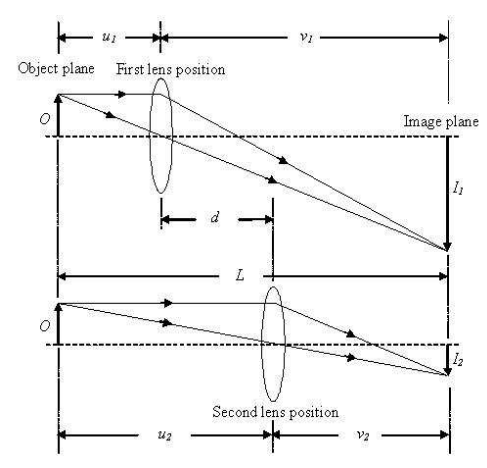
\includegraphics[width=0.50\linewidth, height=0.23\textheight]{Bessel}
\caption{Determination of focal length by using Bessel's Method}
\label{fig:Bessel}
\end{figure}
\newpage
\textbf{Virtual Object Method}
\\
Virtual object method is useful when we want to find focal length of a diverging lens. In virtual object method we need a converging lens which focal length is known and a divergent lens of unknown focal length. Note that in this method relationship between focal length's of converging and diverging lenses is important. Converging lens should be satisfy the following equations
\begin{center}
{\Large 	$\frac{1}{f_{converging}}\textgreater \mid \frac{1}{f_{diverging}}\mid$}
\end{center}
If this requirement is not satisfy then real image will not be formed because the rays of the diverging lens will diverge. The equation of the virtual object method is
\begin{center}
	{\Large $\frac{1}{f_{diverging}}=\frac{1}{s'_{i}}-\frac{1}{s_{i}-d}$}
\end{center}
where $s_{i}$ is the distance between the first screen position and converging lens, $s'_{i}$ is the distance between the second screen position and diverging lens.




























\chapter{Data and Results}
\section{Thin Lens Formula Method}
\begin{table}[h]
\begin{center}
\begin{tabular}{|c|c|c|}
	\hline Object Distance $s_{0}$ & Image Distance $s_{i}$ & Focal Length $f_{m}$\\ 
	\hline 15.6 cm & 13.9 cm & 7.35 cm \\ 
	\hline 12.1 cm & 21.1 cm & 7.69 cm \\ 
	\hline 11.5 cm & 22.0 cm & 7.55 cm \\ 
	\hline 
\end{tabular} 
\end{center}
\caption{Sample data for Thin Lens Formula Method}
\end{table}
As we know from theory section of the experiment, the focal length for a thin lens is equal to
\begin{center}
	$\frac{1}{f_{m}}=\frac{1}{s_{o}}+\frac{1}{s_{i}}$
\end{center}
For first trial: $\frac{1}{f_{m}}=\frac{1}{15.6 cm}+\frac{1}{13.9cm}$ then $f_{m}=7.35$ cm\\
For second trial: $\frac{1}{f_{m}}=\frac{1}{12.1 cm}+\frac{1}{21.1cm}$ then $f_{m}=7.69$ cm\\
For third trial: $\frac{1}{f_{m}}=\frac{1}{11.5 cm}+\frac{1}{22cm}$ then $f_{m}=7.55$ cm\\\\
Average focal length, $\bar{f}$, length is equal to $\bar{f}=(f_{1}+f_{2}+f_{3})/3$. Therefore our average focal length will be
\begin{center}
	$\bar{f}=\frac{7.35 cm+7.69cm+7.55cm}{3}$\\
\end{center}
\begin{center}
	\framebox[70pt]{$\bar{f}=7.42$ cm}
\end{center}
After finding the average focal length we need to find error.
\begin{center}
	$\Delta\bar{f}=\sqrt{\frac{(f_{1}-\bar{f})^{2}+(f_{2}-\bar{f})^{2}+(f_{3}-\bar{f})^{2}}{n-1}}$
\end{center}
\begin{center}
	$\Delta\bar{f}=\sqrt{\frac{(7.35-7.42)^{2}+(7.69-7.42)^{2}+(7.55-7.42)^{2}}{3-1}}$
\end{center}
\begin{center}
	$\framebox[80pt]{$ \Delta \bar{f}=0.22$ cm}$
\end{center}
Note that the real focal length of lens was 7.50 cm. That is why, our error is acceptable.

\section{Bessel Method}
\begin{table}[h]
\begin{center}
	\begin{tabular}{|c|c|c|}
	\hline  $d$ &  $D$ & Focal Length $f_{m}$ \\ 
	\hline 28.8 cm & 46.6 cm & 7.52 cm \\ 
	\hline 24.1 cm & 42.4 cm & 7.17 cm \\ 
	\hline 31.0 cm & 49.1 cm & 7.41 cm \\ 
	\hline 
	\end{tabular} 
\end{center}
\caption{Sample data for Bessel Method}
\end{table}
In this part d is correspond to distance between convergin lenses and D is correspond to distance between object and screen. For Bressel method we are going to use $f_{m}=\frac{D^{2}-d^{2}}{4D}$ as focal length formula.\\\\
For first trial: $f_{m}=\frac{46.6^{2}-28.8^{2}}{4\cdot46.6}$ then $f_{m}=7.52$ cm\\
For second trial: $f_{m}=\frac{42.4^{2}-24.1^{2}}{4\cdot42.4}$ then $f_{m}=7.17$ cm\\
For third trial: $f_{m}=\frac{49.1^{2}-31.0^{2}}{4\cdot49.1}$ then $f_{m}=7.41$ cm\\\\ 
Average focal length, $\bar{f}$, length is equal to $\bar{f}=(f_{1}+f_{2}+f_{3})/3$. Therefore our average focal length will be
\begin{center}
	$\bar{f}=\frac{7.52 cm+7.17cm+7.41cm}{3}$\\
\end{center}
\begin{center}
	\framebox[70pt]{$\bar{f}=7.37$ cm}
\end{center}
Then error will be
\begin{center}
	$\Delta\bar{f}=\sqrt{\frac{(7.52-7.37)^{2}+(7.17-7.37)^{2}+(7.42-7.37)^{2}}{3-1}}$
\end{center}
\begin{center}
	$\framebox[80pt]{$\Delta\bar{f}=0.18$ cm}$
\end{center}
Note that for section 2.1 and 2.2 same lens used. That is why our real focal length is 7.50 cm. Results that obtained from 2.1 and 2.2 are very similar. Therefore there is no certain discrepancy. Error causes will be discussed in discussion and conclusion section.
\newpage
\section{Virtual Object Method}
\begin{table}[h]
\begin{center}
	\begin{tabular}{|c|c|c|c|}
	\hline $s_{i}$ & $s'_{i}$ & $d$ & Focal Length $f_{m}$ \\ 
	\hline 17.3 cm & 14.5 cm & 10.0 cm & -14.7 cm \\ 
	\hline 14.6 cm & 25.3 cm & 5.2 cm & -14.95 cm \\ 
	\hline 22.5 cm & 14.6 cm & 15.0 cm & -15.42 cm \\ 
	\hline 
\end{tabular} 
\end{center}
\caption{Sample data for Virtual Object Method}
\end{table}
In this part we used two different lenses, diverging lens and converging lens. Converging lens's real focal length is 7.5 cm and diverging lens's real focal length is -15.0 cm. In this part $s_{i}$ is correspond to distance between converging lens and first screen position, $s'_{i}$ is correspond to distance between diverging lens second screen position, $d$ is correspond to distance between converging lens and diverging lens.\\\\
For virtual image method we are going to use $f_{diverging}=\frac{s'_{i}(s_{i}-d)}{s_{i}-(s'_{i}+d)}$ as focal length equation. Note that when we want to use virtual object method following equation should be satisfied;
\begin{center}
	$\frac{1}{f_{converging}}\textgreater \mid \frac{1}{f_{diverging}}\mid$
\end{center}
For first trial: $f_{diverging}=\frac{14.5(17.3-10.0)}{17.3-(14.5+10.0)}$ then $f_{diverging}=-14.7$ cm\\
For second trial: $f_{diverging}=\frac{25.3(14.6-5.2)}{14.6-(25.3+5.2)}$ then $f_{diverging}=-14.95$ cm\\
For third trial: $f_{diverging}=\frac{14.6(22.5-15.0)}{22.5-(14.6+15.0)}$ then $f_{diverging}=-15.42$ cm\\\\
Like previous parts, we are going to use same average focal length formula
\begin{center}
	$\bar{f}=\frac{-14.7 cm-14.95cm-15.42cm}{3}$\\
\end{center}
\begin{center}
	\framebox[85pt]{$\bar{f}=-15.02$ cm}
\end{center}
Then error will be
\begin{center}
	$\Delta\bar{f}=\sqrt{\frac{(-14.7+15.02)^{2}+(-14.95+15.02)^{2}+(-15.42+15.02)^{2}}{3-1}}$
\end{center}
\begin{center}
	$\framebox[80pt]{$\Delta\bar{f}=0.37$ cm}$
\end{center}
Real focal length of diverging lens is 15.0 cm. Our focal length error is 0.37 cm and when look at experimental results error is reliable. There is no certain discrepancy. Error causes will be discussed in discussion and conclusion section. 





\chapter{Discussion and Conclusion}
\textbf{1. What are the possible errors in the experiment?}\\
The first possible error should causeb by measurement. In the experiment setup, lowest quantity of distance is about 0.1 cm. Since we measured the distances with our eyes and pencils we should have some errors caused by this. If we had a ruler, we would have betten results than this. Another error cause was chromatic aberration. As we know chromatic aberration is a type of distortion which is a failure of the lens to focus all colors to same point. In the experiment we have observed blur parts around the screen.\\\\
\textbf{2. What kind of approximations did you take into consideration while you were obtaining the physical quantities and how do they affect your results?}\\
Chromatic aberration and scale of experiment setup were main causes of error. During the experiment we approximate the distances to closest point. Working in a dark room was not an easy job if you have problem with scaling of the lenses and screen.\\\\
\textbf{3. What discrepancies did you encounter between the calculated quantities and theoretical or literature values?}\\
As we know our theoretical focal length for converging lens is 7.5 cm and theoretical focal length for diverging lens is 15.0 cm. According to our calculations, we have an average focal length as 7.42 cm for converging lens in part A and 7.37 cm in part B. Besides we have an average focal length for diverging lens as 15.02 cm. If we calculate the percentage error we can determine the discrepancies.

\begin{center}
	$PercentageError=\frac{Theoretical Value-Experimental Value }{Theoretical Value}\times\%100$
\end{center}
For part A: Percentage Error=$\frac{7.50-7.42}{7.50}\times\%100$=\%1.07 cm\\
For part B: Percentage Error=$\frac{7.50-7.37}{7.50}\times\%100$=\%1.80 cm\\
For part C: Percentage Error=$\frac{15.0-15.42}{15.0}\times\%100$=\%2.08 cm\\
Apperantly there is no certain discrepancies that we have encountered in the experiment. Our percentage error is very low. Then we can say this results are valid.\\\\
\textbf{4. What is your overall conclusion?}\\
I think that experiment was successful. We used experiment setup properly. Our experimental results are very close to theoretical ones. We covered the main idea and objectives of the experiment. Chromatic aberration, scaling problem and human error affect the results. However, error percentage can be acceptable. 











\chapter{Application}
\textbf{The Microscope}\\\\
The microscope is device which invented by Galileo in 1610. The microscope is a magnifier. A simple microscope consist of two lenses; the objective which has a very short focus and the ocular or eyepiece which has a longer focus [5]. As we know aberration is an huge problem for image quality. That is why both lenses contains several element those reduce the aberration effect.  
\begin{figure}[h]
\centering
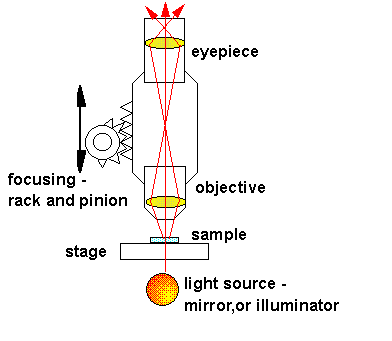
\includegraphics[width=0.4\linewidth, height=0.2\textheight]{microscope}
\caption{Principles of the microscope}
\label{fig:microscope}
\end{figure}
In the microscope, the object is located just outside the focal point of the objective. This led to formed a real image. Then ocular or eyepiece see this image as object. Large virtual image forms by the ocular. Most of microscopes have a turret nose. This turret nose mostly contains three different lenses. Thanks to 3-turret nose system observer can see the same object in three different scale.











\chapter{References}
$[1]$ Loshin, David S. \textit{The Geometrical Optics Workbook.} Boston: Butterworth-Heinemann, 1991. 87.\\\\
$[2]$ Katz, Milton. \textit{Introduction to Geometrical Optics.} River Edge, NJ: World Scientific, 2002. 93.\\\\
$[3]$ Fowles, Grant R. \textit{Introduction to Modern Optics. 2nd Ed.,} Dover ed. New York: Dover Publications, 1975. 295,297.\\\\
$[4]$ "Laws of Lenses." Accessed March 3, 2015. $http://site.iugaza.edu.ps/hele\\gla/files/2010/02/Laws-of-lenses.pdf$\\\\
$[5]$ Jenkins, Francis A., and Harvey Elliott White. \textit{Fundamentals of Optics. 4th ed.} New York: McGraw-Hill, 2001. 200.
























































































\end{document}          
